%
% LaTeX template Masters thesis at IITB
%
% Created by Lakshya Kumar
%
% The official requirement has been persisted with, even if some things could look better some other way.
% Tamper with any of the settings as you see fit and, more importantly, as your guide sees fit.
% Most sections have comments. A lot of stuff is explained in Chapter 1 regarding how to use this template.
% Code snippets for inserting figures, tables and equations are also there in Chapter 1
% Hopefully, this will make report making a little easier.
%

% OK. Here goes.

% Preamble

% Official font size is 12. I thought 11 looked better.
% A4 paper size
% Template for one sided printing of the thesis
\documentclass[12pt, a4paper, oneside]{book}

% Set of packages included. These are all the packages I required, maybe some would be unnecessary and some might be missing. 
% Add any new packages you use over here.
\usepackage{enumitem}
\usepackage{etex}
\usepackage[utf8]{inputenc}
\usepackage{setspace}
\usepackage{amsmath,amsfonts,amssymb,amscd,amsthm,xspace}
\usepackage{titlesec}
\usepackage{vmargin}
\usepackage{fancyhdr}
\usepackage{geometry}
\usepackage{caption}
\usepackage{subcaption}
\usepackage{multirow}
\usepackage{multicol}
\usepackage{url}
\usepackage{tikz}
\usepackage{tabularx}
\usepackage{epstopdf}
\usepackage{graphicx}
\usepackage{booktabs}
\usepackage{rotating}
\usepackage{listings}
\usepackage{framed}
\usepackage{xcolor}
\usepackage{pgfplots}
\usepackage{verbatim}
\usepackage{amsmath}
\usepackage{adjustbox}
\usepackage[linesnumbered,ruled,vlined]{algorithm2e}
\usepackage{algorithmic}
 %\usepackage{floatrow}%
% Define bar chart colors
\definecolor{bblue}{HTML}{000000}
\definecolor{ggreen}{HTML}{909497}
\definecolor{rred}{HTML}{ 515A5A }
\definecolor{ppurple}{HTML}{000000}

%\usepackage[centerlast,small,sc]{caption}
\usepackage[square, numbers, comma, sort&compress]{natbib} % Standard reference style with [3], [4] type numbers in the text and entries sorted according to order of appearance in the References
\usepackage[pdfpagemode={UseOutlines},bookmarks=true,bookmarksopen=true,bookmarksopenlevel=0,bookmarksnumbered=true,hypertexnames=false,colorlinks,linkcolor={black},citecolor={black},urlcolor={black},pdfstartview={FitV},unicode,breaklinks=true]{hyperref}
\hypersetup{urlcolor=black, colorlinks=true} % colors hyperlinks in blue - change to black if annoying

% Math operator definition - may not be required
% If any new operators are required, defien them here
\DeclareMathOperator*{\argmin}{argmin}

\title{\thesisTitle}
\author{\authorName}
\date{\today}

% Currently chapter title has been centered, to left align the chapter title and number, change \centering to \flushleft
\titleformat{\chapter}[display]
  {\normalfont\huge\bfseries\centering}
  {\chaptertitlename\ \thechapter}{18pt}{\Huge}

\setmarginsrb   { 3.0cm}  % left margin
                { 1.5cm}  % top margin
                { 2.0cm}  % right margin
                { 2.2cm}  % bottom margin
                { 0.3cm}  % head height
                { 1.2cm}  % head sep
                { 0.3pt}  % foot height
                { 1.0cm}  % foot sep
                
\newcommand{\ie}{i.\,e.~}
\newcommand{\Ie}{I.\,e.~}
\newcommand{\eg}{e.\,g.~}
\newcommand{\Eg}{E.\,g.~}

% End of the Preamble

% Actual document begins
\begin{document}

\newcommand{\HRule}{\rule{\linewidth}{0.5mm}} % New command to make the lines in the title page

% Import all the variable values from Details.tex
% This file contains all the user specific things that need to be changed such as the thesis title, author name etc. 


\newcommand{\thesisTitle}{Model Based Security Testing for Web Applications}

\newcommand{\degree}{\textbf{Master of Technology (M.Tech)} }

\newcommand{\authorName}{\textbf{Anbarasan K}}

\newcommand{\rollNo}{\textbf{163050071}}

\newcommand{\dept}{Department of Computer Science \& Engineering}

\newcommand{\college}{Indian Institute of Technology Bombay}

\newcommand{\currentyear}{2018}

\newcommand{\currentmonth}{June}

\newcommand{\supervisorOne}{\textbf{Prof. R.K. Shyamasundar}}

\newcommand{\supervisorTwo}{Prof. Supervisor Two}

\newcommand{\examinerOne}{\textbf{Prof. G. Sivakumar}}

\newcommand{\examinerTwo}{\textbf{Prof. Bernard L. Menezes}}

\newcommand{\chairman}{Prof. Chairman}

% Use roman page numbering style (i, ii, iii, iv...) for the pre-content pages
\frontmatter

% Line spacing of 1.5 as per IIT requirement. If you think it looks too spaced out, use 1.3
% I think 11 pt font with 1.3 spacing looks quite good
\setstretch{1.5}

% Import all the pages in the front matter
% This file contains the templates for the first few pages of the thesis including 
% 1. Title page
% 2. Dedication
% 3. Dissertation approval
% 4. Declaration of authorship
% 5. Abstract


%   1. TITLE
\newcommand{\titlePage}{

% No page number
\thispagestyle{empty}
\begin{center}
% thesis title
\vspace*{15px}
{\Huge\bfseries \thesisTitle}\\[1.0cm] 

% submitted in partial fulfillment etc.
%\text{M. Tech. Dissertation}

\textit{Submitted in partial fulfillment of the requirements of the degree of\\[0.2cm] \degree}\\[1.0cm]
 
% author
\textit{by}\\[0.2cm]
\authorName \\[0.2cm] \textit{\textbf{Roll no.}} \rollNo \\[2.0cm]

% supervisor
\textit{Supervisor:}\\[0.2cm]
% or
% \textit{under the supervision of}\\[0.2cm]
\supervisorOne \\[2.0cm]

% iit-b logo

\includegraphics[width=0.25\textwidth]{iitb_logo.jpg}

\vspace*{5px}
% department and college
\dept\\
\college\\
% year
\currentyear\\[0.1cm] 
\end{center}
\clearpage
}
%   2. DEDICATION
%\newcommand{\dedication}{
%\thispagestyle{empty}
%\vspace*{75px}
%\begin{center}\large{\textit{Dedicated to ...}}\end{center}

%\clearpage
%}
%   3. DISSERTATION APPROVAL

\newcommand{\approval}{
% if you use a dedication, then use a page number with the plain page style
\thispagestyle{plain}
% else, use no page number with the empty page style
%\thispagestyle{empty}


% page title
\begin{center}{\huge\bf Dissertation Approval\par}\end{center}

\vspace*{15px}

\noindent This project report entitled 
% title
\textbf{``\thesisTitle"}, submitted by 
% author
\authorName ~(Roll No.  \rollNo), is approved for the award of degree of 
% degree
\degree 
~in 
% branch
Computer Science \& Engineering.\\[1.0cm]
% examiners and supervisors
\vspace*{35px}
\begin{center}
\rule{150pt}{2pt}\\
\textbf{Prof. R.K. Shyamasundar}\\
Dept. of CSE, IIT Bombay\\
Supervisor\\[1.5cm]
\end{center}
\vspace*{10px}
\noindent \rule{150pt}{2pt} \hfill \rule{150pt}{2pt}\\
\textbf{Prof. G. Sivakumar} \hfill \textbf{Prof. Bernard L. Menezes}\\
Dept. of CSE, IIT Bombay \hfill Dept. of CSE, IIT Bombay\\
External and Internal Examiner \hfill Internal Examiner\\[1.0cm]

\vspace*{30px}
\noindent \textbf{Date:} ...... \currentmonth { } \currentyear\\[0.3cm]
\textbf{Place:}\quad\rule{0.4\textwidth}{.3pt} 

% start a new page
\clearpage
}

%   4. DECLARATION OF AUTHORSHIP
\newcommand{\authorship}{
\thispagestyle{plain}

\begin{center}{\huge\bf Declaration of Authorship\par}\end{center}

\vspace*{15px}

% institute declaration text
\noindent I declare that this written submission represents my ideas in 
my own words and where others' ideas or words have been included, I have adequately cited and 
referenced the original sources.  I also declare that I have adhered to all principles of academic 
honesty and integrity and   have   not   misrepresented   or   fabricated   or   falsified   
any   idea/data/fact/source   in   my submission.  I understand that any violation of the above 
will be cause for disciplinary action by the Institute and can also evoke  penal action from the 
sources which have thus not been properly cited or from whom proper permission has not been taken when needed.

\vspace*{15px}

% signature
\begin{flushright}
{Signature: ......................................\\[0.4cm]}

% author name
{\textbf{\authorName}\\[0.0cm]\rollNo\\[2.0cm]}

\end{flushright}
% date
\begin{flushleft}
{Date: ...... \currentmonth { } \currentyear\\}
\end{flushleft}


% start a new page
\clearpage 
}

%   5. ABSTRACT
\newcommand{\abstractpage}{
\thispagestyle{plain}

% header-type text for the abstract - optional
% \small {\noindent\authorName/ \supervisorOne{ }(Supervisor): \textbf{``\thesisTitle"}, \textit{MTech Project}, \dept, \college, \currentmonth { } \currentyear.}\\[0.0cm]
% \HRule\\[0.2cm]


% \vspace*{10px}

\begin{center}{\huge{\textit {Abstract}}\par}\end{center}

\vspace*{10px}

% Abstract text - Type abstract here

Testing of web applications would have become manageable if we had a functional specification of web applications. Due to the underlying issues with browsers and applications being patched regularly it is almost impossible to set realistic functional specifications and system specifications. Thus, vulnerability scanners to test web security will result in false positives, or false negatives. The above disadvantages can be circumvented by model-based testing approach. In this dissertation, we propose a method for web application security using model-based testing approach. The proposed method has been implemented and tested. Model-based testing approach is adapted as it is easy to automate the testing process, and adaptive to changes. Some of the modelling tools like WebSphinx, and PHP-Crawler generate a model based on the static elements in web page. Modern web applications are dynamic in nature due to AJAX technology. Our approach, uses crawljax, a open source modelling tool, and generates a model based on dynamic event handler, then generates test cases for security based on the model of the web application, and execute them in a browser to validate the model for security vulnerabilities. Our case study of DVWA-Damn Vulnerable Web Application that contains security vulnerabilities has shown advantages of our tool approach. We have performed experiments with our test framework in a sample space of 15 web applications. We opine that our testing tool is capable of capturing security vulnerabilities like XSS and SQL Injection in the tested web applications in an automated manner.


% Index terms
% \noindent \textbf{Index terms}: Sentiment 

% Start a new page
\clearpage 
}

\titlePage

\setcounter{page}{1}
% \dedication

\addcontentsline{toc}{chapter}{Dissertation Approval}
\newgeometry{lmargin=1cm,rmargin=1cm}
\begin{figure}[hbtp]
    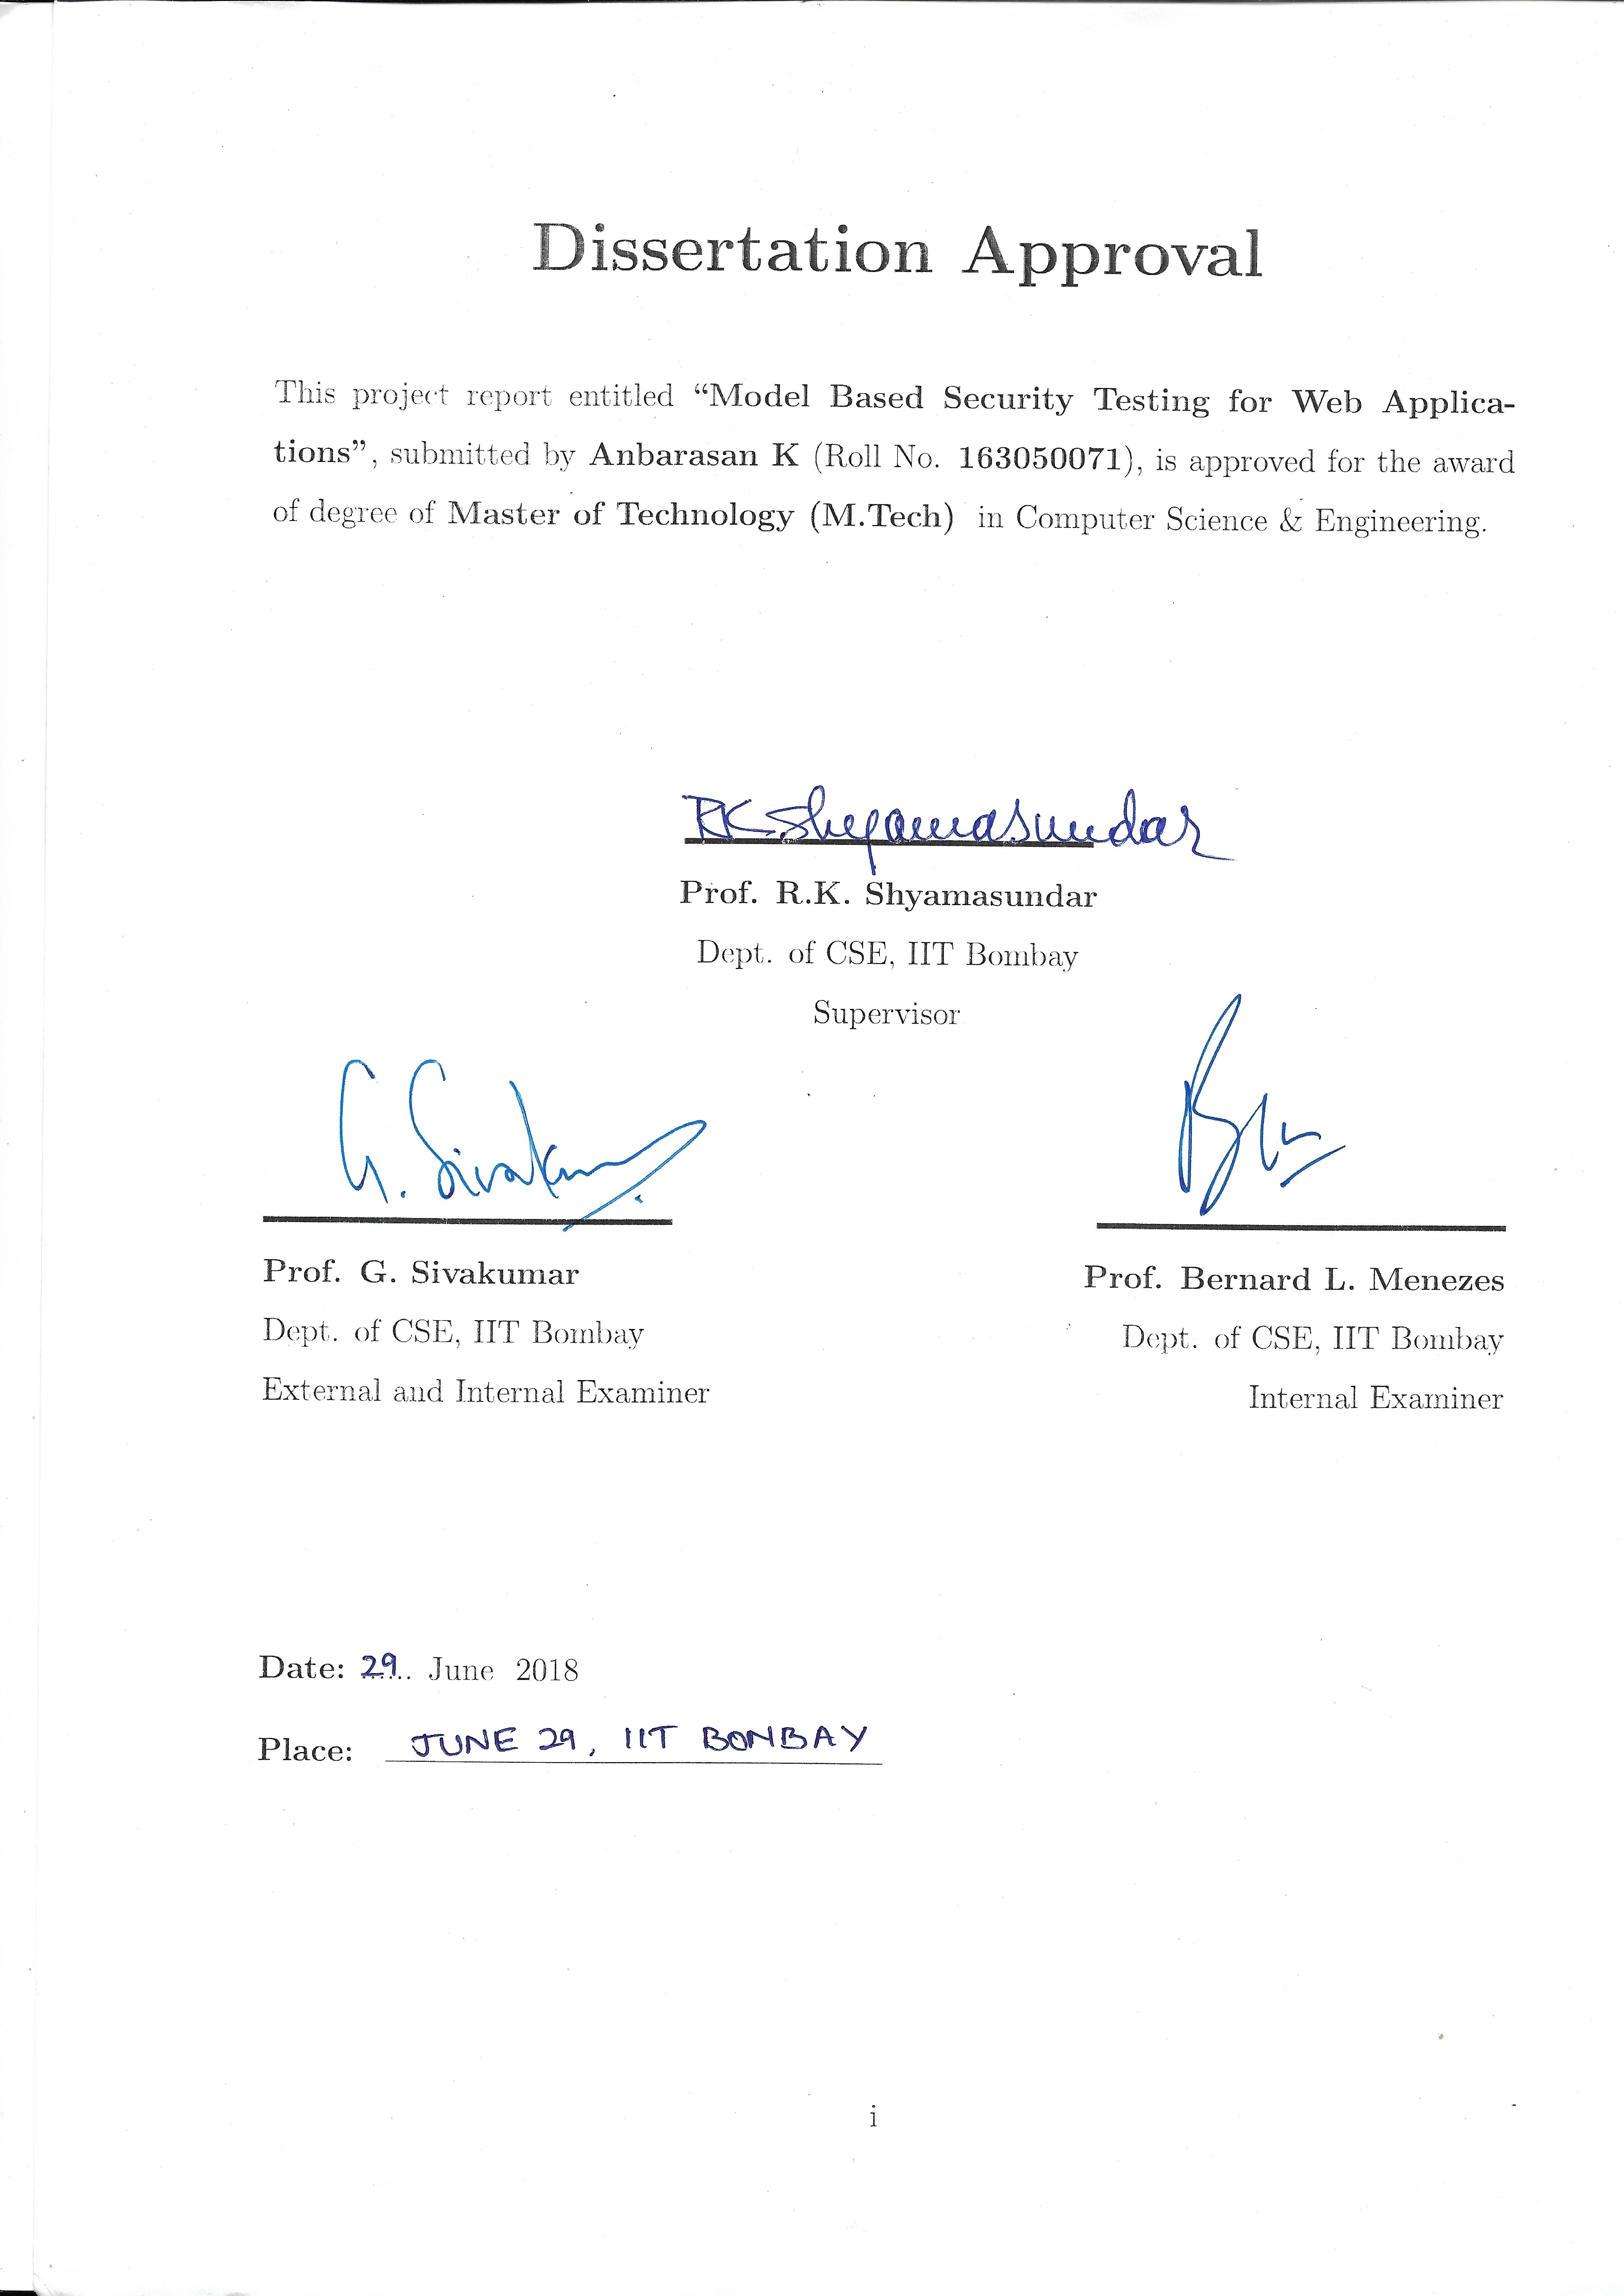
\includegraphics {Approval.jpg}}
\end{figure}
\restoregeometry
\clearpage

\addcontentsline{toc}{chapter}{Declaration of Authorship}
\newgeometry{lmargin=1cm,rmargin=1cm}
\begin{figure}[hbtp]
    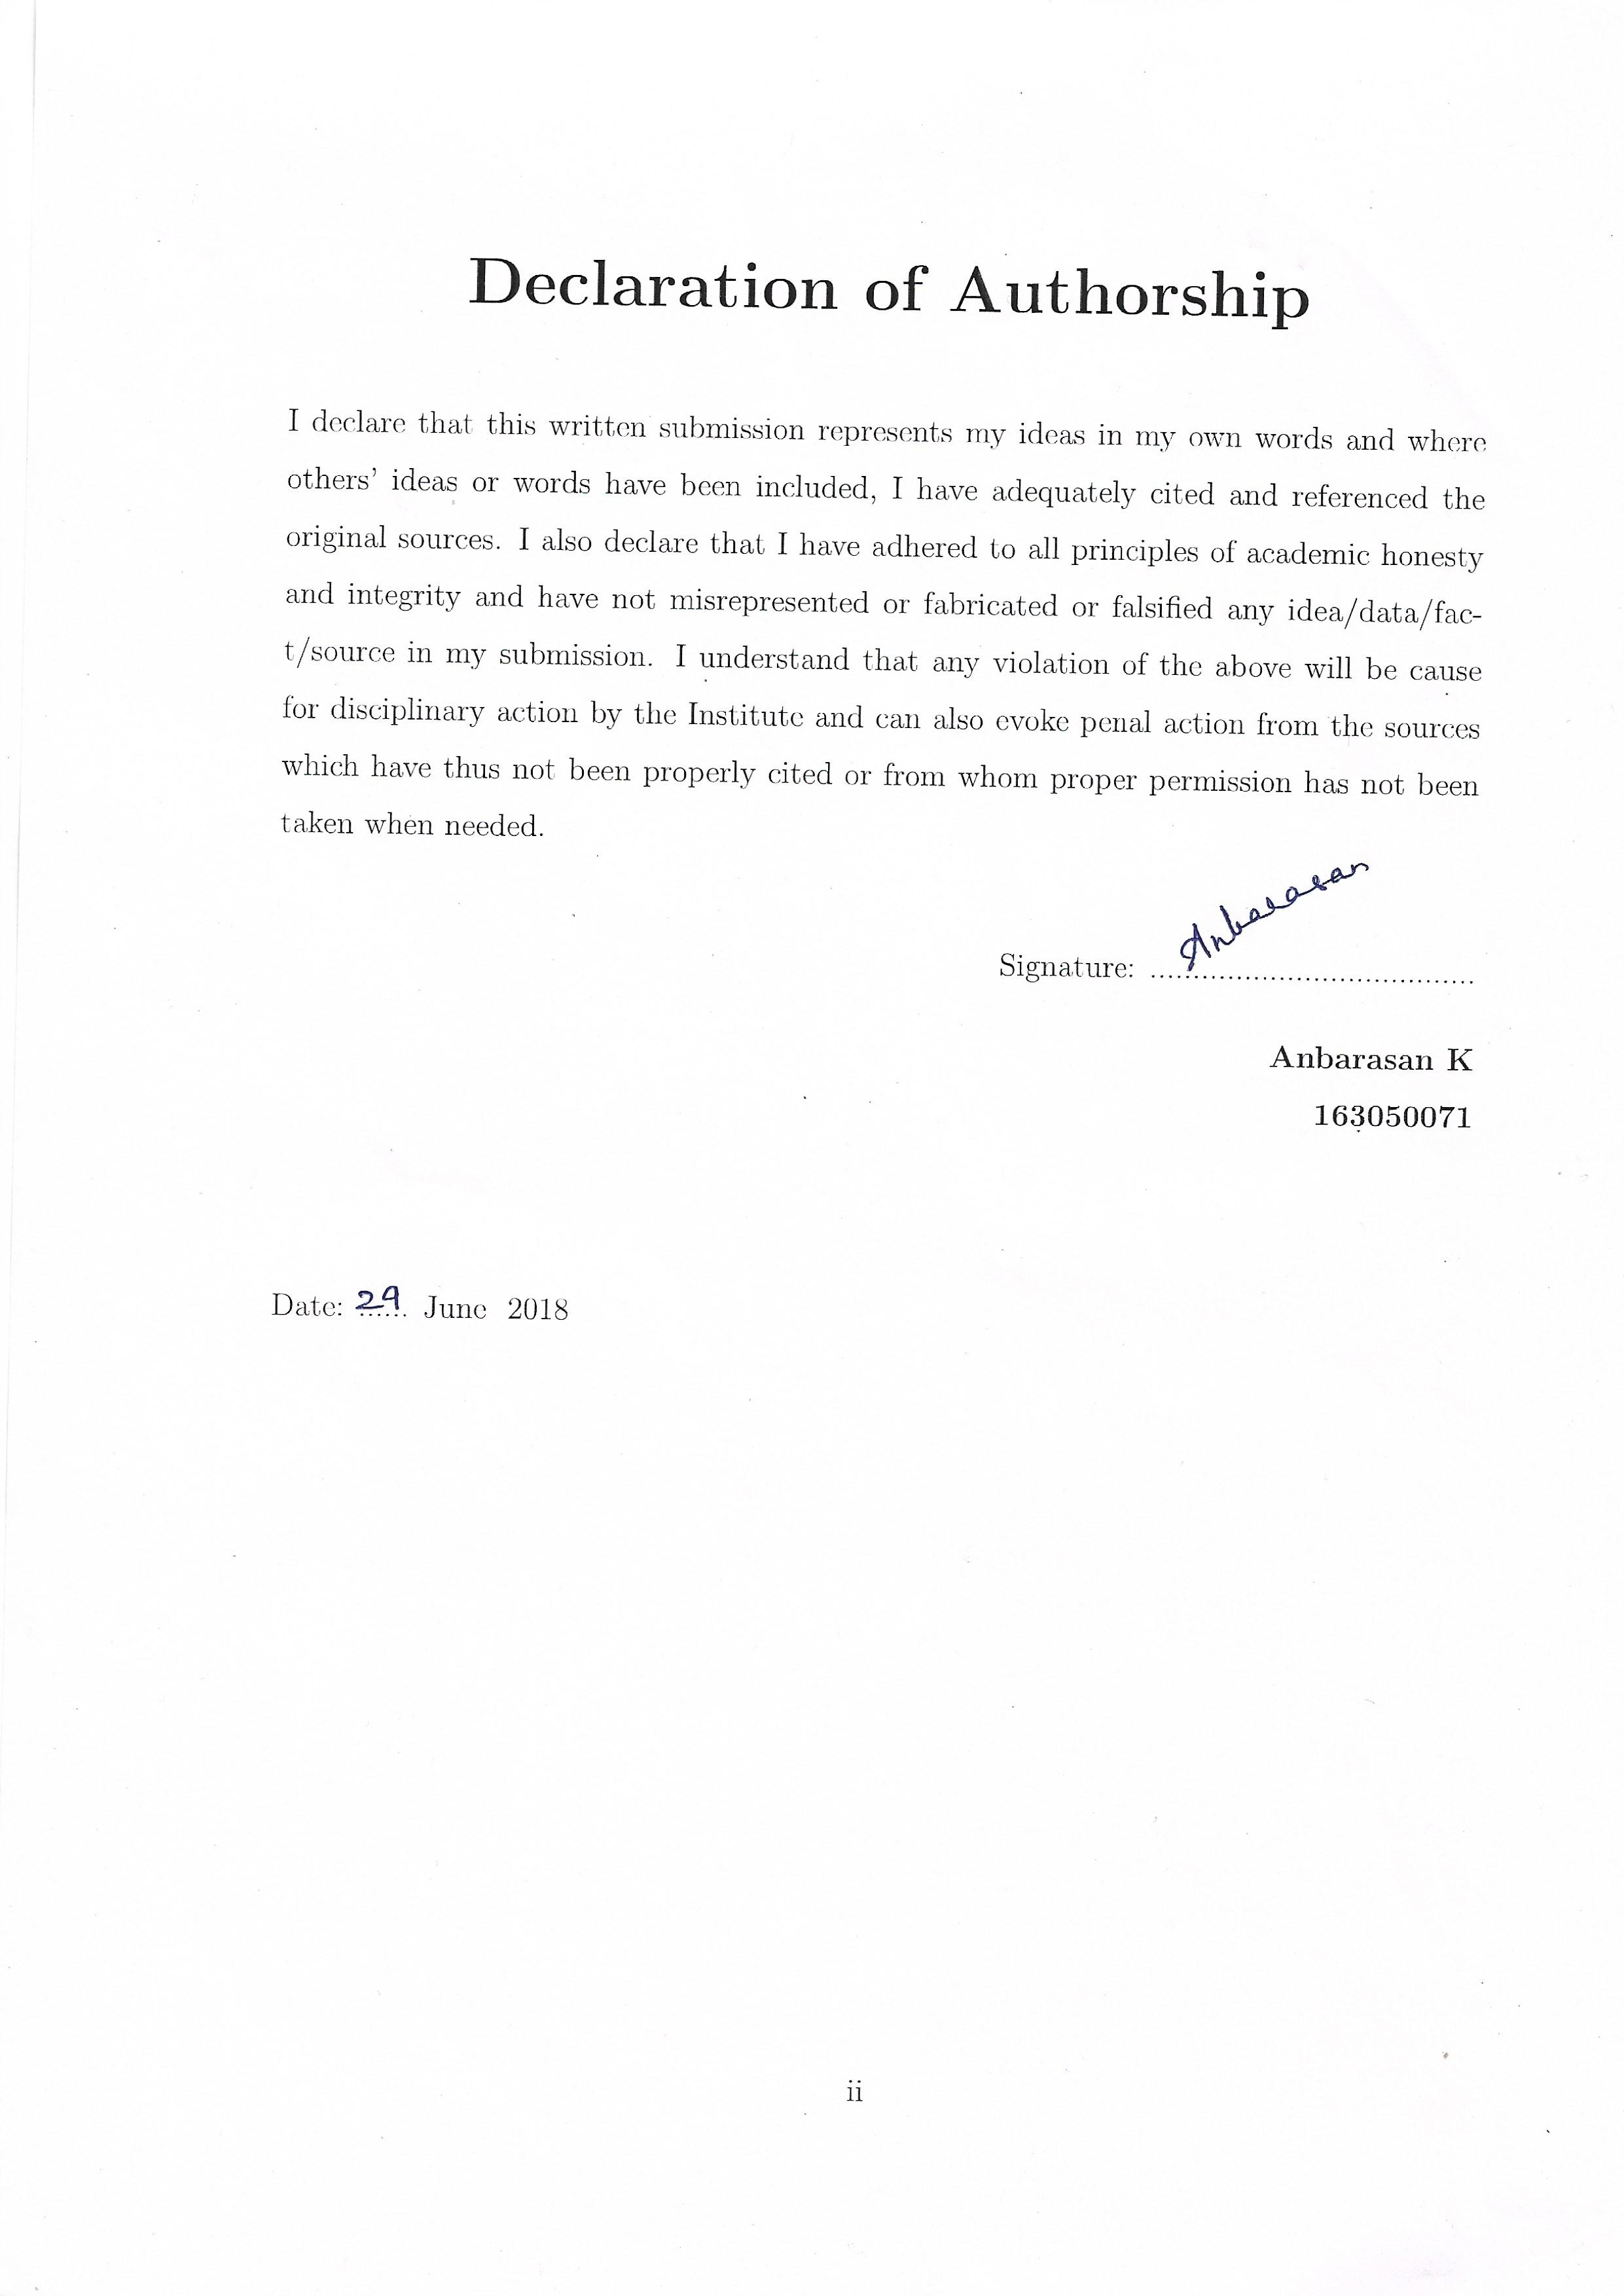
\includegraphics {Author.jpg}}
\end{figure}
\restoregeometry
\clearpage
\addcontentsline{toc}{chapter}{Abstract}
\abstractpage

\pagestyle{fancy}

% Set the left side page header to "Contents"
\lhead{\emph{Contents}} 

% Write out the Table of Contents
\tableofcontents 

% Set the left side page header to "List of Figures"
\lhead{\emph{List of Figures}} 

% Write out the List of Figures
\listoffigures 
\addcontentsline{toc}{chapter}{List of Figures}

% Set the left side page header to "List of Tables"
% \lhead{\emph{List of Tables}} 

% Write out the List of Tables
% \listoftables
% \addcontentsline{toc}{chapter}{List of Tables}

\fancyhead{}
\rhead{\thepage}


% Use arabic page numbering style (1, 2, 3...) for the body of the report
\mainmatter

% Import the Chapters
% Introduction

% Main chapter title
\chapter{INTRODUCTION}
\label{chap:intro}

\section{Web Applications}
Web Applications are application programs that are stored in remote servers and delivered over the Internet using browser interfaces. The user interface of web applications are built using the interplay of HTML, CSS and JavaScript. Javascript being a highly dyanamic language, web applications are dynamic with interactive elements and some applications require server side processing. Web Applications require a server to handle client requests and a database to store the information. Web Applications include e-commerce websites, online forms, content management systems and email programs[1]. 

\section{Security Testing}
With the increasing complexity of web systems, and more content moving from offline to online platform, security testing has become a critical activity of web application development life cycle. The focus of security testing of web applications is to maintain the confidentiality of data, prevention against information leakages. This is performed by checking web application behaviour on injecting malicious data. Security Testings aids in exposing security vulnerabilities like XSS, SQL Injection, file inclusion, URL injection[3]. 

\section{Web Application Modelling}
A model is an abstraction or simplification of the behavior of the application under test(SUT). The model is captured in a machine with the purpose of acting as a test sequence (trace) generator. The model represents the architecture of the web application. A web application can be modelled using finite State machine or labelled transition system approaches[7]. 

\section{Model Based Testing}
Model-based testing is a technique for designing and executing applications to perform testing (includes Test cases to be executed on every object in the model). In Model Based Testing, test cases are generated automatically and systematically from the model of the system under test. There are three step in Model based Testing. Firstly, a model of the SUT is built from informal requirements or from the functionality of the SUT. Secondly, execution traces of the model are used to generate test cases. Since there can be infinitely many/long execution traces be present, test selection criteria is applied reduce the testcases. Lastly, using the test model and the test selection criteria, Test cases are derived for model based testing[7]. 

\section{Model Based Security Testing}

Model based testing can be adapted to test security of web applications. Model based testing for functionality usually generates positive test cases for validation of web applications. To perform security testing, negative test cases and attack scenarios have to be derived. Attack scenarios include generation of malicious code or data to retrieve unauthorized data from the web server. This involves two steps- Modeling activity to capture the behavioral aspects and/or architecture of the web application. The next step is to define the test purposes- in this case to test the security in particular the type of attack on web security.   
 

\chapter{PROBLEM STATEMENT}

The growth of Internet and evolution of web application technologies has led to the vulnerabilities in security- data confidentiality, data integrity and service availability. Manual testing of security in web applications is time consuming and its difficult to perform in case of regression testing. Web Vulnerability scanners can be used to detect vulnerabilities but they often led to generation of false positive and false negative results. A desirable solution to perform security testing is automated security testing. 
Automated security testing has its challenges in terms of deriving proper functional behavior of the web applications. This is due to the lack of proper documentation of web applications or various technologies used for developing web applications. Modern web applications are no more static but dynamic due to the extensive use of javascript and CSS. With javascript, functionalities can be added in the client side of the web applications which makes calls to the server using (Asynchronous javascript) AJAX. These calls needs to be validated and tested thoroughly to prevent information leaks. 

\newline
To overcome the above difficulties in security testing of application, there is a need of method for automated testing of vulnerabilities of software that can be realized testing it with a model can overcome the above challenges. This approach is called model based security testing. We derive a model for web applications handling AJAX(Javascript and XML) calls and test security vulnerabilities based on the testcases derived from model.

\newline
The thesis is organized as follows:\\
Chapter 3- Literature Survey, Chapter 4- Web Application Security Vulnerabilities, Chapter5- Our approach of modelling web applications for security testing, Chapter 6- Modelling of Web Applications via State Machine Chapter 7- Security Test Framework, Chapter 8- Experimentation and Results, Chapter 9- Related Work, Chapter 10- Conclusion and Chapter 11- Future Work

Existing approaches like SQLMap performs security testing without out a model. Our approach being model driven provides exhaustive coverage of testing web applications.

\chapter{LITERATURE SURVEY}

In this chapter, we give a brief overview of the existing tools for web testing.

\section{WebMate: A Tool for Testing Web 2.0 Applications}

Webmate[1] is a functional testing tool for Web 2.0 applications. Webmate automatically crawls through the Web applications performing regular application testing as well as cross browser compatibility testing. The input to the webmate tool is the url of the website to test and it creates a usage model by crawling and triggering user actions with a javascript event handler. This usage model is extracted and different browsers and the model is compared with a reference model to capture cross-browser compatibility issues. Webmate also checks for HTML and CSS for browser specific issues. Results of the tests are reported back to the tester. Webmate approach as opposed to manual testing generates testcases automatically for functional testing of web applications. 

\section{Search-based security testing of web applications}

Biofuzz[3], search-based security testing tool proposes a blackbox testing technique to inject malicious SQL data to detect SQL Injection vulnerabilities. It injects malicious SQL query in form inputs and based on the feedback of SQL query it detects whether the attack is successful. It identifies target input parameters such as form input fields, and generate form inputs to ther server. The tool Biofuzz, is bound to MYSQL database and PHP as server. Biofuzz tool finds all the input fields with a crawler to detect input fields vulnerable to SQL attacks. It uses evolutionary algorithms to mutate the SQL inputs to test all possible combinations of SQL queries. 


\section{Crawling AJAX-Based Web Applications through Dynamic Analysis}
Crawling AJAX is more difficult than classical multi-page web applications. In Multi-page web appliations, each page has a unique URL assigned to them but with AJAX pages are dynamic which multiple content can be assigned to same URL. Extraction of hyperlinks and creating a model does not accurately represent the architecture of web applications. Instead of hyperlinks javascript handle can be used to navigate the application and create a model. The web applications are dynamically represented through the Document Object Model(DOM). The User Interface changes are accurately represented by DOM changes instead of URL changes[4,5].


\section{Issues with existing tools}

Webmate is model based testing tool only for functionality testing of web applications. The security testing feature is not offered. MBVT Tool is a model based vulnerability testing tool but it requires functional specification of web applications for its model and realizing a functional specification for web applications is not feasible because of web application being regularly patched.
%\input{Chapters/Chapter03_02}

\chapter{WEB APPLICATION SECURITY VULNERABILITIES}

In this chapter, we provide an overview of the most prevalent security vulnerabilities(among top 10 vulnerabilities) in web applications.[8]

\section{XSS-Cross Site Scripting}
Cross-Site Scripting or XSS[6] is one of the most prevelant security attacks in the world.Cross Site scripting or XSS attack targets end-users. User input fields such as form field, url parameter, cookie are vulnerable to XSS attacks. The fields are  used by the server to produce responses. An attacker can inject malicious data using a script, usually written in JavaScript, which will be executed by an end-user browser through the input fields in web applications. If the input fields are not validated and sanitized for malicious scripts, then the web applications are vulnerable to attack.  

\subsection{Reflected XSS-Cross Site Scripting}
In reflected XSS attacks[6], the malicious script is executed immediately and response containing malicious requests is provided to the end-user. This kind of attack is non-persistent and affect the user executing script in fields such as a search box query or the user clicking a link from a malicious URL. Spam emails containing the malicious URL or Javascript can also initiate a Reflected XSS attack. The attack is performed using a single request and response. This attack is possible in web application where the user data inputs are not properly encoded or the special characters used in scripts are not properly filtered.

\subsection{Stored XSS-Cross Site Scripting}
Stored XSS attack[6] is a kind of attack in which malicious script is injected into the web application database using methods like injecting in a comment box in a forum or posting data using input fields.In stored XSS attacks, the malicious script is saved in the application's database permanently and hence known as persistent XSS attack. This attack affects all the users loading from the database and hence more dangerous than Reflected XSS in terms of scale. When an end user loads the web application containing Stored XSS scripts, if the data from database is not properly sanitized or filtered the javascript is executed in the browser and sensitive information such as session ids are exposed to the attacker.  


\section{SQL Injection}

SQL injection or SQLI[6] is an attack that uses malicious SQL code for backend database manipulation to access information that was not intended to be displayed to the normal end user. This database information may include any number of items, including sensitive company data, user lists or user private data.A successful SQLI attack can result in the unauthorized viewing of user lists, the deletion of entire tables in database and, database administrative rights being granted to the end user. An attacker in SQL injection manipulates a standard SQL query to exploit non-validated input(user input fields) vulnerabilities in a database. 

\chapter{OUR APPROACH FOR MODELLING \\WEB APPLICATIONS FOR SECURITY TESTING}

In this chapter, we discuss our modelling techniques for assessing security for web applications. Creation of a model of a web application requires traversing all paths from the home page of web application to all links present in the web page. Transitions from a web page happens due to static hyperlinks and dynamic javascript events in a webpage(ex. onclick() events). Model of a web application security testing needs to capture all the elements in a webpage and all transitions possible from the webpage. The following sections illustrate our approach to model the web application.

\section{Document Object Model(DOM) Tree}

The Document Object Model (DOM) is a programming interface(API) for HTML and XML documents. It represents the document structure, style and content of web applications. DOM is represented as nodes and objects in the document. A Web page is a document encoded in HTML(XML). This document is displayed in the browser window as an application. The DOM is an object-oriented representation of the web page, which can be modified in the web applications with JavaScript.In DOM representation, every HTML element is considered as an object. The DOM represents the web page as a tree structure of HTML tags.

An example DOM Tree is given in the below figure.

\begin{figure}[htpb]
  \begin{center}
    \resizebox{75mm}{50mm} {\includegraphics {Chapters/DOM.eps}}
    \caption {Example of DOM Tree}
  \label{fig:Table}
  \end{center}
\end{figure}

\section{Navigation Graph Model}

In Navigation Graph model[5], a graph is built with nodes and edges where each node represents a Web page and each edge represents a link. It is a model built by a Web crawler (or Web spider) program that automatically traverses the Web application's hyperlink structure and retrieves the content of the Web pages. This model considers only static HTML elements such as hyperlinks and ignore all the dynamic elements such as AJAX elements. In this model, each web page url is a different node and if multiple web pages have the same url(dynamic content) this model does not represent the accurate website structure. \\
\section{Finite State Machine}
In Finite State Machine, since each node represents a different State of an AJAX web page and each edge between nodes represents a transition performed on a clickable element. In a webpage, each element of the page can became clickable at runtime(dynamic). The home web page is defined as the root or start State and new States are added as the application is crawled. To find the clickable elements in a webpage, the DOM model of the web page is extracted and the clickable elements are obtained. These elements are subjected to click events and then the resulting DOM model is obtained. In case there is a change in DOM, then a new State is created and an edge is added between the States.  This crawling procedure is recursively called to find all possible States.

The below figure illustrates a example web application and its corresponding State machine model.

\section{Example of a web application and its state machine}

The below figure represents the web application http://www.testfire.net/

\begin{figure}[!h]
 \begin{center}
    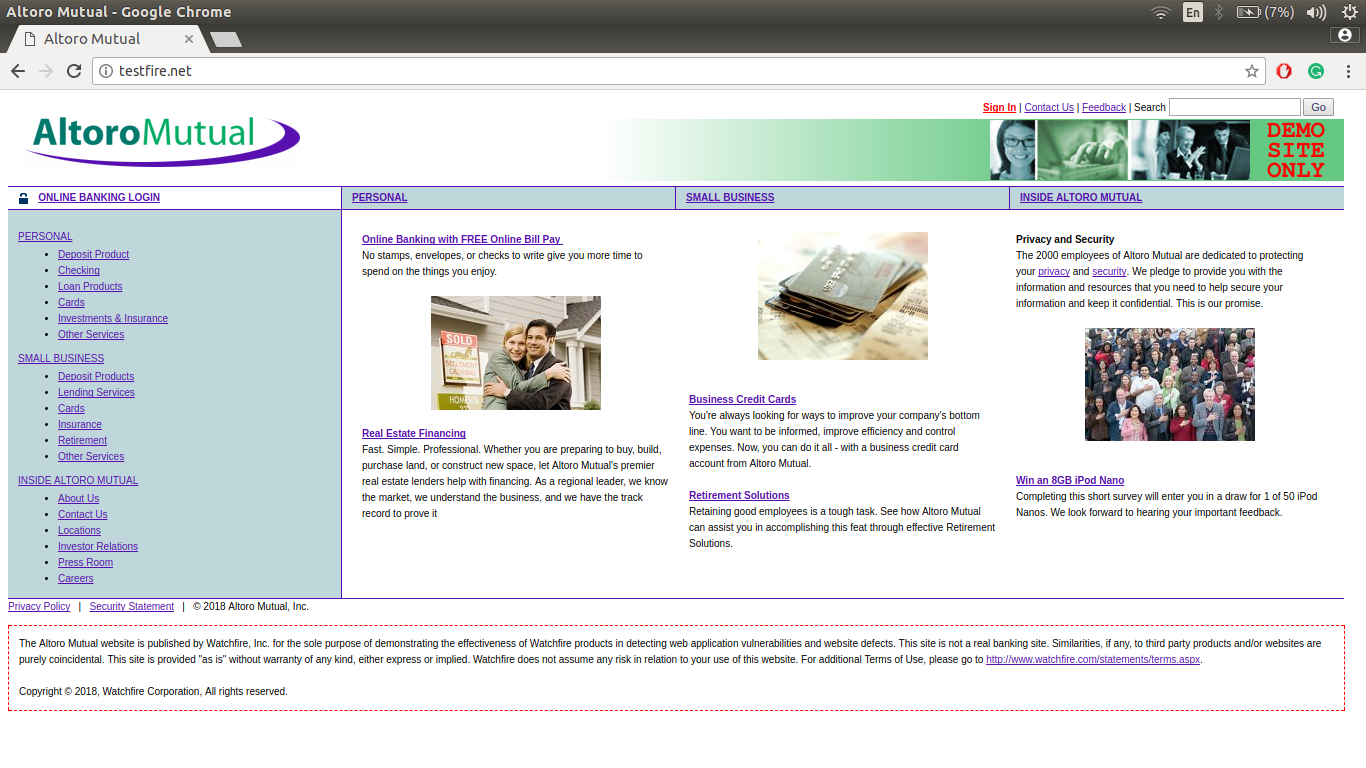
\includegraphics[width=\textwidth]{Chapters/Testfire.eps}} 
    \caption {A example banking web application}
  \label{fig:Table}
 \end{center}
\end{figure}

\subsection{Crawl Level 1}

The below figure is a state machine model for web application http://www.testfire.net/ with crawl level 1. 

\begin{figure}[!h]
 \begin{center}
        \includegraphics[width=\textwidth]{Chapters/Crawl1.eps}}} 
    \caption {State Machine Model for Crawl Level 1}
  \label{fig:Table}
 \end{center}
\end{figure}

\newpage
\section{Choice of the approach used in the dissertation}
Since the model web applications are AJAX based and dynamic in nature, the Finite State Machine Model is better than navigation graph with each node representing the State of DOM. Crawljax is selected as the the crawling tool for modelling web applications. 


\chapter{MODELLING OF WEB APPLICATIONS VIA STATE MACHINE}

\section{Generation of State Machine Model}

 State Machine for a Web Applications is characterized with a three tuple (r, V, E)
 \begin{itemize}
     \item V is the list of vertices which is recognized as the DOM States in the model
     \item E is the edges or transitions associated with States after clicking capable events(candidate elements).
     \item r is the root element or initial State of the model 
 \end{itemize}
 
Crawljax, a open source tool is used to generate the State machine model for web applications. It uses selenium webdriver as a event handler to make direct calls to the browser. The url of web application is the input to create State machine. The browser is intialized and the DOM tree of the web application is extracted and the DOM State is created as the root element. The next step is to find the clickable events in the webpage, both static elements(HTML hyperlinks) and javascript events(eg. Onclick events). These elements are determined as candidate elements for firing transitions in the webpage. Candidate elements are activated one by one and the resulting DOM tree is extracted. The resulting DOM tree is compared with the existing DOM States by the use of a comparator. The DOM tree is converted into strings and the string is the matched with the result State is added to the State machine with an edge added to the previous State. The candidate element from which the transition is done is now removed from the list and the previous State is restored. All the States reachable from the initial State is determined by firing events with all candidate events. This crawl procedure is done for a maximum crawl depth as defined initially.\\
\newline
The below figure illustrates a example web application and its corresponding State machine model.

\section{Example of a Web Application and its Model}

The below figure represents the web application http://www.testfire.net/

\begin{figure}[!h]
 \begin{center}
    \resizebox{100mm}{75mm} {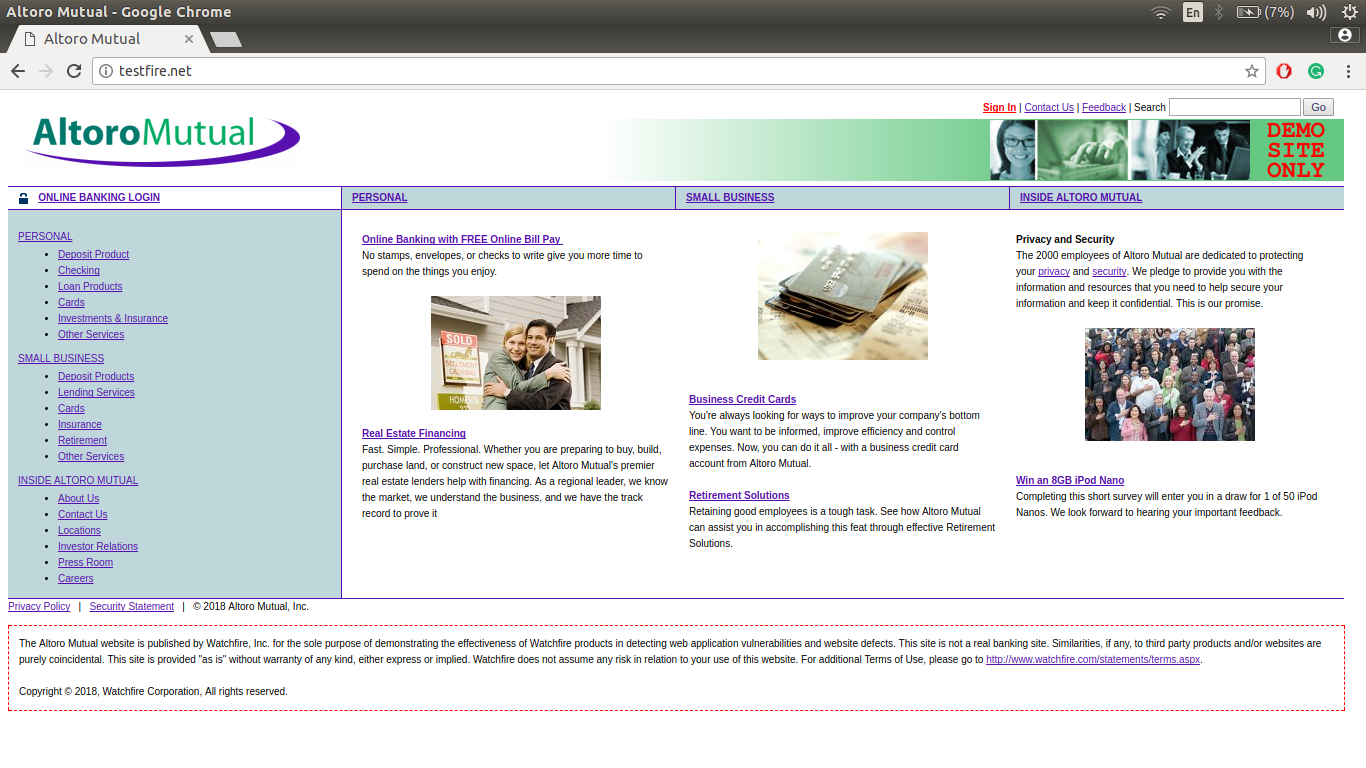
\includegraphics {Chapters/Testfire.eps}}
    \caption {A example banking web application}
  \label{fig:Table}
 \end{center}
\end{figure}

\subsection{Crawl Level 1}

The below figure is a state machine model for web application http://www.testfire.net/ with crawl level 1. In crawl level1, initial start DOM state is home page of web applications and all the state reachable from the start state is modelled.

\begin{figure}[!h]
 \begin{center}
    \resizebox{100mm}{75mm} {\includegraphics {Chapters/Crawl1.eps}}
    \caption {State Machine Model for Crawl Level 1}
  \label{fig:Table}
 \end{center}
\end{figure}

\subsection{Transition between states}
Let us consider the transition between states- start state(index page) to state 39.
\\
$ "from" : "index",
  "to" : "state39" $
  \\

The transition is caused the event type click  through the element submit button having value Go. \\
$
  "element" : "Element{node=[INPUT: null], tag=INPUT, $ \\ $text=, attributes={type=submit, value=Go}}",
  "eventType" : "click" $
\\

The submit button is present in the DOM tree path as show below. \\
$ 
  "id" : "xpath /HTML[1]/BODY[1]/DIV[1]/FORM[1]/TABLE[1]/TBODY[1]/$\\ $TR[1]/TD[2]/INPUT[2]",
 $\\
 
Similarly, the transition between the states- (index page) to state35 can be explained as below.
$
{
  "from" : "index",
  "to" : "state35",
 $\\
 
 The transition is caused by selecting a hyperlink default.aspx?content=security.htm
 $
  "element" : "Element{node=[A: null], tag=A, text=security, $ \\ $attributes={href=default.aspx?content=security.htm}}",
  "eventType" : "click"
}$
\\

The hyperlink is present in the DOM tree path below\\
$
 "id" : "xpath /HTML[1]/BODY[1]/DIV[2]/TABLE[1]/TBODY[1]/$ \\$ TR[2]/TD[2]/SPAN[1]/TABLE[1]/TBODY[1]/TR[1]/TD[3]/A[2]",
 $


\subsection{Crawl Level 2}

 In crawl level 2, the states reachable from start state are captured and the modelling procedure is repeated with these states as starting states unlike crawl level 2. The below figure is a State Machine Model derived from web applications http://www.testfire.net for a crawling level of 2.

\begin{figure}[htpb]
 \begin{center}
    \resizebox{150mm}{125mm} {\includegraphics {Chapters/Crawl2.eps}}
    \caption {State Machine Model for Crawl Level 2}
  \label{fig:Table}
 \end{center}
\end{figure}


\chapter{SECURITY TEST FRAMEWORK}

Architecture for Security test framework is depicted in Figure 7.1. It has been implemented in python using requests library and mechanize browser[8] through an API. Requests are used to send http requests and acquire responses from web applications. Mechanize is a Stateful and headless web browser. Headless web browser or UI less web browser is suited for our purpose because in some cases of browsers with UI like chrome or firefox, browser side security can prevent the security attacks while the web application is still vulnerable to security. Such kind of attacks is made possible in headless browser and it is identified in our experimentation. 

\begin{figure}[htpb]
 \begin{center}
    \resizebox{150mm}{50mm} {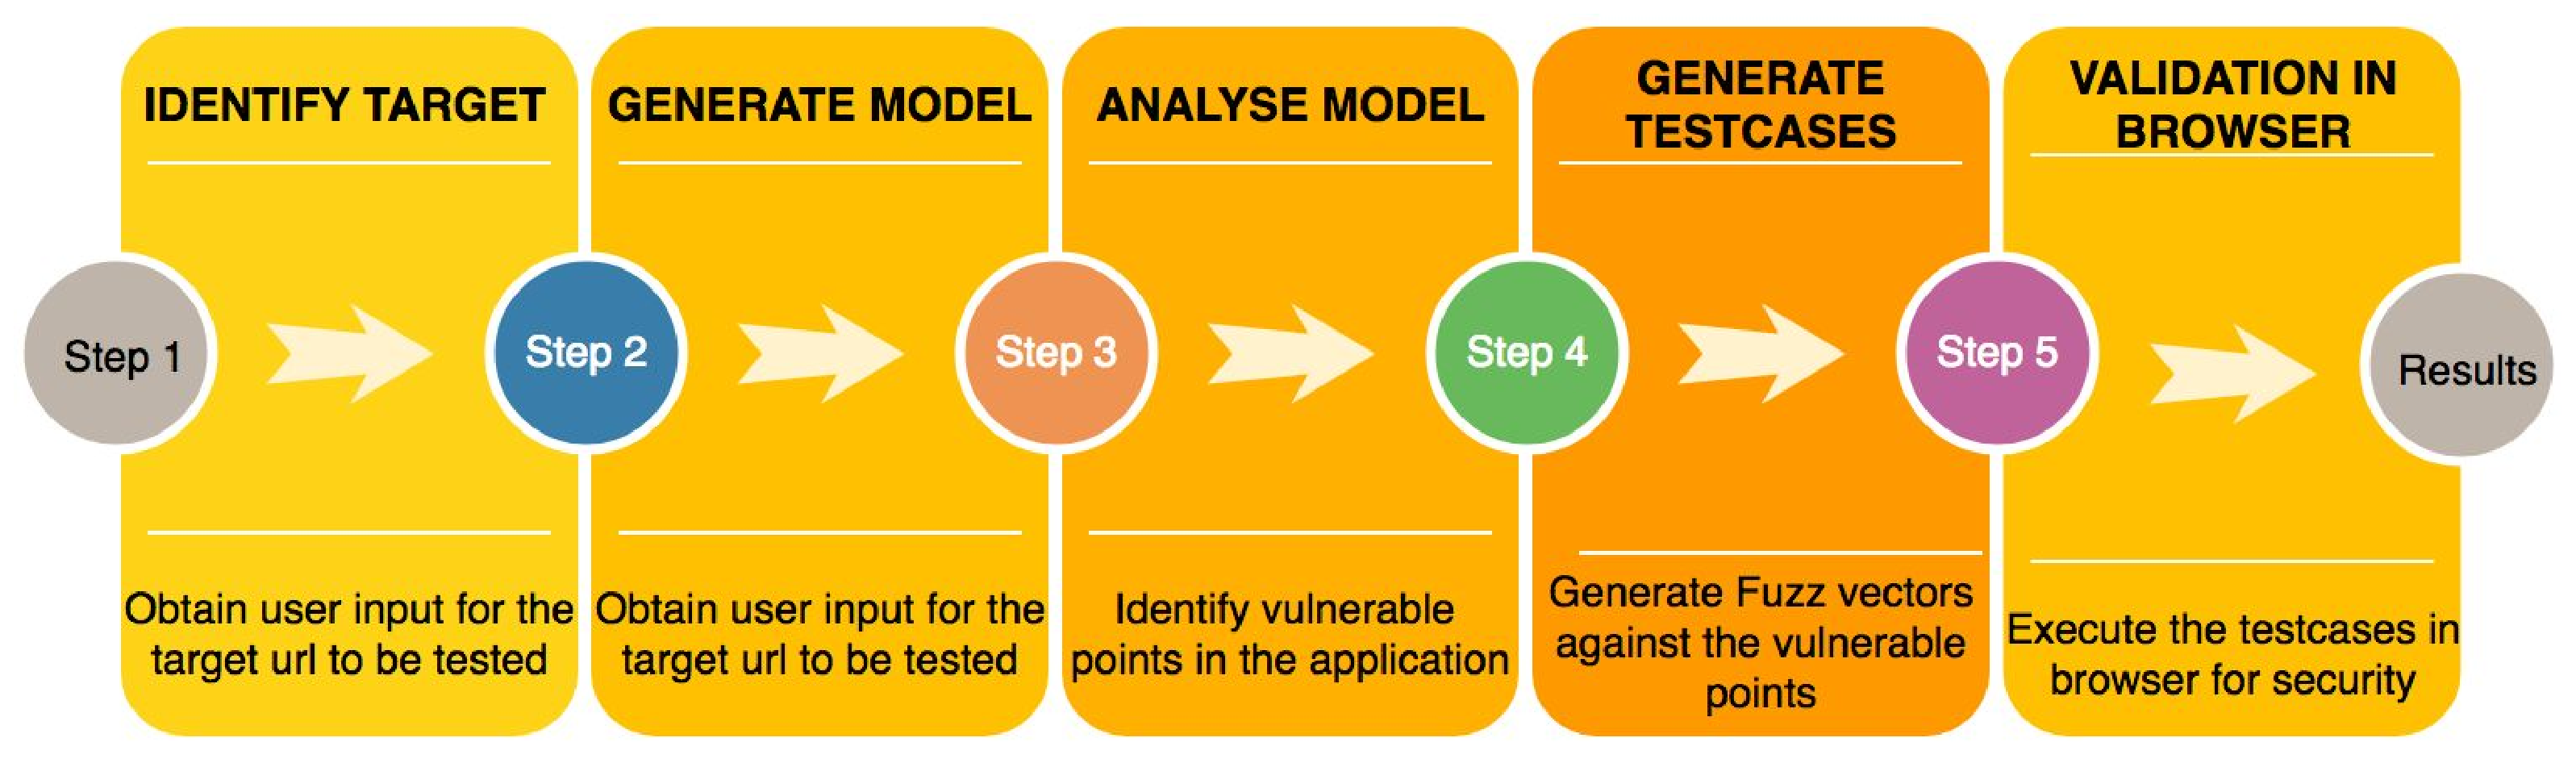
\includegraphics {Chapters/architecture1.eps}}
    \caption {Architecture}
  \label{fig:Table}
 \end{center}
\end{figure}

\section{Identification of Vulnerable points of attack from the model}
The State machine model represents the architecture and the DOM elements of the the web applications. The next step is to define the attack pattern and test objective of Security Testing. The most vulnerable security threats are XSS and SQLI attacks. The candidate elements such as forms fields, user inputs, GET and POST parameters which are vulnerable to these attacks are determined from the the DOM tree extracted in the State Machine model as follows. 
\\
DOM tree of the start state is obtained from the state machine. Tags in the DOM Tree are parsed only by one and user modifiable elements are captured.
Form fields, user inputs, GET/POST parameters and textarea fields, are identified added to a list named as vulnerable elements. Form fields are identified with their tag attribute id. Both the form name and id attributes are added to the list. User Input fields, password field are identified with their tag attribute name. If tag attribute id is not present then tag attribute name is used for input fields identification. Input Elements whose element those are hidden in the web page are also added to the vulnerable elements. All the fields identified as vulnerable elements are stored in a file Vulnerability\_model.
If there are no user modifiable fields, then there are no candidate elements are found for vulnerability for that particular DOM state. The DOM state is marked as visited and the process is repeated for all states in the state machine.. The vulnerability\_model is output to the user as HTML report for all the states.
This analysis is implemented by a parsing the DOM Tree using Beautifulsoup library[9]. \\

Example of Vulnerable fields identified from model;\\

 \\$<input class="loginInput" name="username" size="20" type="text"/>$

 \\$<input autocomplete="off" class="loginInput" name="password" size="20" type="password"/>$

 \\$<input name="Login" type="submit" value="Login"/>$

\section{Test Suite Generation based on the Model}

The vulnerability points are tested for XSS Attacks and SQL Injection attacks. The test cases are generated for these vulnerability points using the following methods.

\subsection{Test Suite Generation for XSS Attack}

Consider a simple model with a webpage having a input element such a search box and a submit button which displays the results of a search query. \\

The webpage http://www.xssgame.com/f/m4KKGHi2rVUN/ is show as below:

\begin{figure}[!h]
 \begin{center}
    \resizebox{100mm}{75mm} {
\includegraphics {Chapters/XSS.eps}}
    \caption {Test Webpage for XSS Attack}
  \label{fig:Table}
 \end{center}
\end{figure}

The test case for XSS attack is derived from the model as follows. \\
State Tested: Start State \\
Target Element: Search Input Box (identified from model)\\
$
<input id="demo2-query" name="query" onfocus="this.value=''" value="Enter query here..."/>$\\
$<input id="demo2-query" name="query" onfocus="this.value=''" value="Enter query here..."/>
$\\
Attack Script: $<script>alert('XSS')</script> $\\
\newline
If the XSS script gets reflected as $<SCRIPT>alert('XSS');</SCRIPT> $ in HTTP Response then the attack has succeeded. This implies there is no filters or input sanitization performed for the attack script. The javascript is executed by the browser.\\
Instead, it it gets displayed as$ &lt;SCRIPT&gt;alert('XSS')</SCRIPT&gt;$ then the attack is not successful, since the special characters of script are escaped and encoded. The javascript will not be executed by the browser.
Similarly the test cases are generated for multiple states, target elements and attacks scripts. The testcases are variants of javascript, execution of javascript embedded in different tags like body, img src. Javascript codes to escape the filters of web application are also part of test cases.
\\
There are two variants of XSS attacks, Persistent or Stored XSS and Non-persistent or Reflected XSS attacks. 
\\
In Non-persistent or reflected XSS attack, the javascript is injected to the user accessing web application but the script is not stored in the web application permanently. For this kind of attack after injecting the code, the resulting HTTP response is verified.
\\
In persistent of stored XSS attacks, the javascript is stored permanently in the database of the web application and the script is executed for all persons who access the web application. For persistent XSS attack, after injecting the script, the HTTP response should be verified and also web application should be loaded again and checked whether the malicious script is loaded. This kind of attack happens when image comment is stored in a web application, or a message is posted in a forum.
\\
Example XSS Attack testcases.
\\
$ <BODY ONLOAD=alert('XSS')>$\\
$<IMG SRC="javascript:alert('XSS')"$\\
$</xmp><script>alert(‘XSS’)</script><xmp>$\\
$<SCRIPT/SRC="http://xss.rocks/xss.js"></SCRIPT>$

\subsection{Test Suite Generation for SQLI Attack}

The objective of SQLI inject testing is to read unauthorized stored data from a database at the back end of web application such as passwords and usernames. The test suite for SQLI attack is generated by deriving SQL queries for retrieving stored data.  The first phase is to find which all input parameters which will flow into the SQL query Statements. These are the SQL queries which are vulnerable to SQLI attacks. Example of input fields are username and password field which which will be translated as a SQL query to validate credentials in the database. The target input fields vulnerable to SQLI attacks are extracted from the State graph model. \\

Consider a web page having input elements such a username and password fields.

\begin{figure}[!h]
 \begin{center}
    \resizebox{100mm}{75mm} {\includegraphics {Chapters/SQLI.eps}}
    \caption {Test Webpage for SQLI Attack}
  \label{fig:Table}
 \end{center}
\end{figure}


\\
The sample test case for SQL Injection attack is as follows. 
\\
State Tested: Root DOM State (identified from state machine)\\
Target Element: password Field  (identified from state machine)\\
$
<input class="loginInput" name="username" size="20" type="text"/>$\\
$<input autocomplete="off" class="loginInput" name="password" size="20" type="password"/>$
\\
Attack SQL Query: 1 OR 2=2\\
\newline
Entering a username and password into the query will flow into the database as USERNAME="uname" and PASSWORD="pwd". With the attack SQL Query 1 OR 2=2. SQL Query will flow as USERNAME="uname" and PASSWORD="1" OR 2=2.
If the web application does not have security measures to control the attack the password check will be bypassed and application will login. If the resulting response contains invalid password then the attack is successful else the password check is bypassed and attack is successful.
\\
\newline
Similarly the test cases are generated for all the states, target elements and SQL Injection queries.
\\
\newline
Example SQL Injection Attack testcases.\\
$‘TEST$\\
$SELECT VERSION();$\\
$1' OR '1'='1$\\
$1'1$\\
$1 AND 1=1$\\
$1' AND 1=(SELECT COUNT(*) FROM tablenames); --$\\
$1' AND non_existant_table = '1$\\
$OR username IS NOT NULL OR username = '$\\

 \\
\section{Fuzzing Based Techniques for Test Suite Generation}

Fuzz Testing is a software testing technique in which invalid or random generated data called fuzz is created. In our tool, the attack vectors are generated using The steps for fuzz testing include the basic testing steps. The steps for fuzz testing include the basic testing steps-

\begin{itemize}
\item Identify the target DOM State.
\item Identify GET/POST parameters and user input fields vulnerable to security flaws
\item Generate Fuzzed attack vectors using recursive fuzzing, bruteforce fuzzing and replacive fuzzing techniques.
\end{itemize} 

We employ replacive fuzzing by replacing the special characters which can be escaped by their hexadecimal codes. Replacive fuzzing is employed by changing the user modifiable parameters reflected in the URLs of states in the state machine.

\section{Validation of the attack pattern from model in Browser}

 The target parameters and testcases are derived from the model as explained in above sections. 

Target parameters:

$
<input id="demo2-query" name="query" onfocus="this.value=''" value="Enter query here..."/></xmp>$\\
$<input id="demo2-query" name="query" onfocus="this.value=''" value="Enter query here..."/>$
\\
$
<input class="loginInput" name="username" size="20" type="text"/>
<input autocomplete="off" class="loginInput" name="password" size="20" type="password"/>
$
 
XSS Attack testcases.
\\
$ <BODY ONLOAD=alert('XSS')>$\\
$<IMG SRC="javascript:alert('XSS')"$\\
$</xmp><script>alert(‘XSS’)</script><xmp>$\\
$<SCRIPT/SRC="http://xss.rocks/xss.js"></SCRIPT>$\\
\newline
SQL Injection Attack testcases.\\
$‘TEST$\\
$SELECT VERSION();$\\
$1' OR '1'='1$\\
$1'1$\\
$1 AND 1=1$\\
$1' AND 1=(SELECT COUNT(*) FROM tablenames); --$\\
$1' AND non_existant_table = '1$\\
$OR username IS NOT NULL OR username = '$\\
 \newline
The execution framework is implemented in python using Requests Library and Mechanize browser. Mechanize is a headless browser, browser without UI and it is suited for our purpose because browsers like firefox, chrome has security mechanisms implemented with them and they can block attack scripts and provide false negatives. But the web application may be still vulnerable to security attacks. Requests library is used to load content from the web application, the requested content is intercepted. The target parameters identified from the model are now injected with malicious scripts from testcases in the intercepted content. Browser object is created for mechanize browser. The intercepted content is now submitted to the mechanize browser using the browser object created.\\
\newline
The resulting HTTP response from the web application is stored in a debug.log file. The resulting HTTP response from the debug.log file is now analysed whether the injected script is executed. If the HTTP Response contains the injected javascript without filters then it implies the reflected XSS attack is possible.  If the elements cannot be modified, the response is obtained as the element is read only. This implies the attack is not successful. For stored XSS attack, after injecting the script, open the browser web application again through a different browser object and find whether the web application contains the injected code. For SQL Injection attacks, if the resulting HTTP response contains data from the web application database, the attack is successful. For malformed SQL queries, if the HTTP response contains any syntax error or database error or database version is obtained, the attack is successful since the SQL query gets executed is not filtered by the web application. If the SQL query is not executed and if the HTTP response contains invalid input, attack is not successful.\\

The output obtained is written into a summary file for all the states whether the attack is successful or not.
 

\\In the next chapter, we shall illustrate our framework with a CASE study.

\chapter{EXPERIMENTAL RESULTS}

In this chapter, we shall highlight the results of security vulnerabilities on various web applications. 

\section{Case Study Coverage- DVWA Web Application}

Let us consider a case study of web application named Damn Web Vulnerable Web Application for our Model Based Security Testing Approach.

DVWA-Damn Web Vulnerable Application is a PHP/MySQL application which contains security vulnerabilities such as SQL Injection, Reflected XSS and Stored XSS Attacks. There are three security levels - low, medium and high with decreasing order or security vulnerabilities across the levels. The framework is tested against DVWA tools across the security levels.
\\
The below figure depicts the Damn Vulnerable Web Application\\
\newpage
\begin{figure}[!h]
 \begin{center}
    \resizebox{100mm}{75mm} {\includegraphics {Chapters/DVWA1.eps}}
    \caption {State Machine Model of DVWA}
  \label{fig:Table}
 \end{center}
\end{figure}


\section{State Machine Model of DVWA web application}

The first phase of our case study is to generate a state machine model for Web application. The Figure 8.1 illustrates the state machine model generated for the application DVWA for crawl level 1. Also the number of states and their url is depicted in the Table 8.1

\begin{figure}[!h]
 \begin{center}
    \resizebox{100mm}{75mm} {\includegraphics {Chapters/DVWA.eps}}
    \caption {State Machine Model of DVWA}
  \label{fig:Table}
 \end{center}
\end{figure}

\begin{table}[!h]
\centering
\caption{State Generated in Model}
\label{State Generated in Model}
\begin{tabular}{||c | c||}
\hline
/dvwa/vulnerabilities/sqli/                & state9,  \\
/dvwa/vulnerabilities/sqli/                & state9,  \\
/dvwa/vulnerabilities/csrf/                & state6,  \\
/dvwa                                      & index,   \\
/dvwa/vulnerabilities/exec/                & state5,  \\
/dvwa/vulnerabilities/fi/?page=include.php & state8,  \\
/dvwa/vulnerabilities/captcha/             & state7,  \\
/dvwa/instructions.php                     & state2,  \\
/dvwa/vulnerabilities/brute/               & state4,  \\
/dvwa/setup.php                            & state3,  \\
/dvwa/vulnerabilities/xss\_s/              & state13, \\
/dvwa/vulnerabilities/xss\_r/              & state12, \\
/dvwa/vulnerabilities/upload/              & state11, \\
/dvwa/vulnerabilities/sqli\_blind/         & state10, \\
/dvwa/login.php                            & state17, \\
/dvwa/about.php                            & state16, \\
/dvwa/phpinfo.php                          & state15, \\
/dvwa/security.php                         & state14 \\
\hline

\end{tabular}
\end{table}

\newpage

\section{Points of vulnerability identified from Model}

The second phase of our automated test tool is identifying the points of vulnerability from the model. 
It is done by analyzing the  state machine model and by parsing the DOM Tree for parameters which require user inputs(GET/POST parameters) form fields, hidden inputs, parameters than can be modified. These parameters are identified as target parameters which are vulnerable for security attacks.

\newline
\textbf{Vulnerability fields for XSS and SQL Injection}

\newline
\textbf{State9}

$<input name="id" type="text"/>$

$<input name="Submit" type="submit" value="Submit"/>$

\newline
\textbf{State17}

 $<input class="loginInput" name="username" size="20" type="text"/>$

 $<input autocomplete="off" class="loginInput" name="password" size="20" type="password"/>$

 $<input name="Login" type="submit" value="Login"/>$

\newline
\textbf{State13}

$<input maxlength="10" name="txtName" size="30" type="text"/>$

$<input name="btnSign" onclick="return checkForm();" type="submit" value="Sign Guestbook"/>$


\newline
\textbf{State10}

$<input name="id" type="text"/>$

$<input name="Submit" type="submit" value="Submit"/>$

\newline
\textbf{State4}

$<input name="username" type="text"/>$

$<input autocomplete="none" name="password" type="password"/>$

$<input name="Login" type="submit" value="Login"/>$

\newline
\textbf{State11}

$<input name="MAX$\_$FILE$\_$SIZE" type="hidden" value="100000"/>$

$<input name="uploaded" type="file"/>$

$<input name="Upload" type="submit" value="Upload"/>$


\newline
\textbf{State7}

$<input name="step" type="hidden" value="1"/>$

$<input autocomplete="none" name="password$\_$new" type="password"/>$

 $<input autocomplete="none" name="password$\_$conf" type="password"/>$

 $<input name="Change" type="submit" value="Change"/>$


\newline
\textbf{State5}

$<input name="ip" size="30" type="text"/>$

$<input name="submit" type="submit" value="submit"/>$

\newline
\textbf{State6}

$<input autocomplete="none" name="password$\_$new" type="password"/>$

$<input autocomplete="none" name="password$\_$conf" type="password"/>$

$<input name="Change" type="submit" value="Change"/>$
 
\newline
\textbf{State12}

$<input name="name" type="text"/>$

$<input type="submit" value="Submit"/>$

\newline
\textbf{State3}

$<input name="create$\_$db" type="submit" value="Create / Reset Database"/>$

\newline
\textbf{State14}

$<input name="seclev$\_$submit" type="submit" value="Submit"/>$

\section{Validation Results of execution in Browser}

The final phase of our tool is presenting the results of execution to the user in a html report. Below are the results of our tool for XSS and SQL Injection security testing.

\newline
\textbf{XSS and SQL Injection Test Results}
\newline
\\
\textbf{State11: }
\newline
No candidate elements for Reflected and stored XSS vulnerability
\newline
No candidate elements for SQL Injection 
\newline
\\
\textbf{State10: }
\newline
No Reflected XSS and stored Vulnerability not found for script
\newline
\textbf{SQL Injection Vulnerability found for payload\\ 
$ 1 UNION ALL SELECT 1,2,3,4,5,6,name FROM sysObjects WHERE xtype = \'U\' -- $}
\newline
\\
\textbf{State14: }
\newline
No Reflected XSS and stored Vulnerability not found for script
\newline
\textbf{SQL Injection Vulnerability found for payload 
\\
$1 AND USER$\_$NAME() = 'usr' $}
\newline
\textbf{State9: }
\newline
No Reflected and stored XSS Vulnerability not found for script
\newline
\textbf{SQL Injection Vulnerability found for payload 
\\
$1 AND ASCII(LOWER(SUBSTRING((SELECT TOP 1 name FROM sysobjects$
\\$WHERE xtype='U'), 1, 1))) > 116 $}
\newline
\\
\textbf{State12:} 
\newline
textbf{Payload Reflected in Response. Reflected XSS Vulnerability found for script
\\ $<SCRIPT SRC=http://ha.ckers.org/xss.js></SCRIPT>$}
\newline
\\
\textbf{State13: }
\textbf{Payload loaded from web application. Stored XSS Vulnerability found
\\$'-alert(3)-'$}

\section{Inference of results from Case Study of DVWA web application}
The DVWA application contains security vulnerabilities like XSS and SQL Injection. Our Test Framework identifies the security vulnerabilities of the web application correctly and identifies which parameters are vulnerable which aids for web developers to correct the security flaws. An exhaustive testing of web application with numerous payloads are tedious to execute by manual testing and also hidden parameters can be overlooked in manual testing. Our tool aids in overcoming these drawbacks and our case study demonstrates our tool usage in security testing.

\begin{table}[h]
\label{Summary of Web Application Tested - DVWA}
\caption{Summary of Web Application Tested - DVWA}
\begin{tabular}[h]{||c | c||}
\hline
Number of states tested                    & 10  \\
Crawl Level configuration                   & 1  \\
Number of elements identified for testing   & 30  \\
Number of elements found vulnerable        & 5 \\
Types of vulnerabilities found             & SQLI, Reflected XSS, Stored XSS  \\
Types of vulnerabilities not found    & CSRF, File Inclusion   \\
\hline

\end{tabular}
\end{table}
Vulnerabilities other than XSS and SQLI like CSRF, File Inclusion are not found as they are beyond scope of our thesis.

\chapter{RELATED WORK}

\begin{table}[!ht]
\caption{Comparison Analysis of Security Testing Tools}
\label{Comparitive Analysis of Security Testing Tools}
\begin{tabular}{|l|l|l|l|l|}
\hline
Features                 & Our Framework & BioFuzz       & MBVT Tool    & WebMate       \\
\hline
Model of the tool        & State Machine & State Machine & UML Diagrams & State Machine \\
\hline
Fuzzing based Technique  & Yes           & Yes           & No          & Yes           \\
\hline
XSS Testing              & Yes           & No            & Yes          & No            \\
\hline
SQLI Testing             & Yes           & Yes           & Yes           & No            \\
\hline
Headless Browser support & Yes           & Yes           & Yes           & No            \\
\hline
Automation               & Yes           & Yes           & Yes          & Yes\\
\hline
\end{tabular}
\end{table}

We have compared our approach with Webmate[1], Biofuzz[3], MBVT Tool[2]. Webmate is a functional testing tool based on model based testing approach without security attributes testing. MBVT Tool uses UML Diagrams as a modelling technique which required generation of UML diagrams based on functional specification. Our tool generates a model without functional specifications. BioFuzz is a search based testing tool which tests only SQL Injection attacks without XSS Testing support. Our tool also performs XSS Testing. Table 9.1 illustrates the comparative analysis of our tool with other model based security testing tools. Apart from these tools there are other tools like SQLMap which tests only for SQL Injection attack. All the tools used fuzzing based technique for generation of testcases with the exception of MBVT.


\chapter{CONCLUSION}

Web application vulnerability scanners generate few false positive and false negative results. This can be avoided by blackbox model based security testing. To model the web application, different types of Web Application modelling techniques is discussed. The State machine model based on DOM tree is chosen as the model for model based testing since it is flexible for modern web applications. Since SQLI and XSS are the most common security threats, these two attack scenarios have been chosen as attack models. The test suite is generated with the architecture model against the attack models. The attack pattern is executed in an automated manner against the web application.

\chapter{FUTURE WORK}
The security test framework in this thesis focus on the major security threat vulnerabilities-XSS and SQL Injection attacks.The current framework does not consider security attacks such as LDAP Injection, Broken Authentication and session Management. The challenges in detecting these attacks are the session IDs and authorization tokes expires within a time frame for web applications and brute force techniques are not effective in discovering these vulnerabilities. The techniques to detect these vulnerabilites are in future scope. Our scope of executing the security testing is within headless browsers and extending it to browsers with UI by bypassing security configurations of browsers is of future scope.

\chapter{REFERENCES}
\begin{enumerate}  
\item WebMate: A Tool for Testing Web 2.0 Applications, Authors: Valentin Dallmeier,Martin Burger, Tobias Orth, Andreas Zeller Journal: JSTools'12, June 13, 2012, China.
  \newblock
\item Model-Based Vulnerability Testing for Web Applications, Conference: Software Testing,Verification and Validation Workshops (ICSTW), 2013 IEEE Sixth International Conference on Authors: Franck Lebeau, Bruno Legeard, Fabien Peureux.
\newblock
\item Search-based security testing of web applications. Authors: Julian Thomé, Andreas Zeller, Alessandra Gorla. Conference: SBST 2014 Proceedings of the 7th International Workshop on Search-Based Software Testing.
\item Crawling AJAX by Inferring User Interface State Changes Authors: Arie van Deursen, Ali Mesbah, Engin Bozdag. Conference: Web Engineering, 2008. ICWE '08. Eighth International Conference
\item A Crawljax Based Approach to Exploit Traditional Accessibility Evaluation Tools for AJAX Applications. Authors: F. Ferrucci1 , F. Sarro1 , D. Ronca1 , S. Abrahao2. Journal: Information Technology and Innovation Trends in Organizations, May 2011.
\item Automatic Creation of SQL Injection and Cross-Site Scripting Attacks. Authors: Adam Kiezun ˙ ,
Philip J. Guo , Karthick Jayaraman , Michael D. Ernst
\item A Survey on Model-based Testing Approaches: A Systematic Review. Authors: Arilo C. Dias, Neto Rajesh, Subramanyan
 Marlon Vieira, Guilherme H. Travassos
\item OWASP Top10 Security vulnerabilities. \\
https://www.owasp.org/index.php/Top\_10-2017\_Top\_10
\item Mechanize Browser API Documentation.\\
http://mechanize.readthedocs.io/en/latest/browser\_api.html
\item Beautiful Soup HTML Parser Documentation.\\
https://www.crummy.com/software/BeautifulSoup/bs4/doc/
\end{enumerate}

\appendix % Cue to tell LaTeX that the following 'chapters' are Appendices

% Import the Appendices
% \input{AppendixA}

\backmatter

% This file contains the templates for the last few pages of the thesis including 
% 1. List of publications
% 2. Acknowledgements

% \newcommand{\publications}{

% Page number at bottom
% \thispagestyle{plain}

% Title
% \begin{center}{\huge{\textbf{List of Publications}} \par}\end{center}

% \vspace*{15px}

% List your publications here

% 1.

% 2.
% }

\newcommand{\acknowledgements}{

% Page number at bottom
\thispagestyle{plain}

% Title
\begin{center}{\huge{\textit{Acknowledgements}} \par}\end{center}

\vspace*{15px}

% Write acknowledgement here

I am thankful to my supervisor Prof. R.K.Shyamasundar for his enormous support and insightful suggestions throughout my project. I am grateful to him for providing me his code base support which was very useful in carrying out my experiments. His insightful suggestions to the various problems that I faced during my project, were not only useful, but also helped me in broadening my basic understanding of project area. 

\vspace*{15px}

\begin{flushright}
{Signature: ......................................\\[0.4cm]}

{\textbf{\authorName}\\[0.0cm]\rollNo\\[2.0cm]}
\end{flushright}

\begin{flushleft}
{Date:} ...... \currentmonth { } \currentyear\\
\end{flushleft}
}

% Bibliography

%\label{Bibliography}
%\lhead{\emph{Bibliography}}


%\bibliographystyle{acl2016.bst} % Use the "unsrtnat" BibTeX style for formatting the Bibliography

%\bibliography{Bibliography} % The references (bibliography) information are stored in the file named "Bibliography.bib"

\clearpage

% List of Publications
% \addcontentsline{toc}{chapter}{List of Publications}
% \publications

\clearpage

% Acknowledgements
\addcontentsline{toc}{chapter}{Acknowledgements}
\newgeometry{lmargin=1cm,rmargin=1cm}
\begin{figure}[hbtp]
    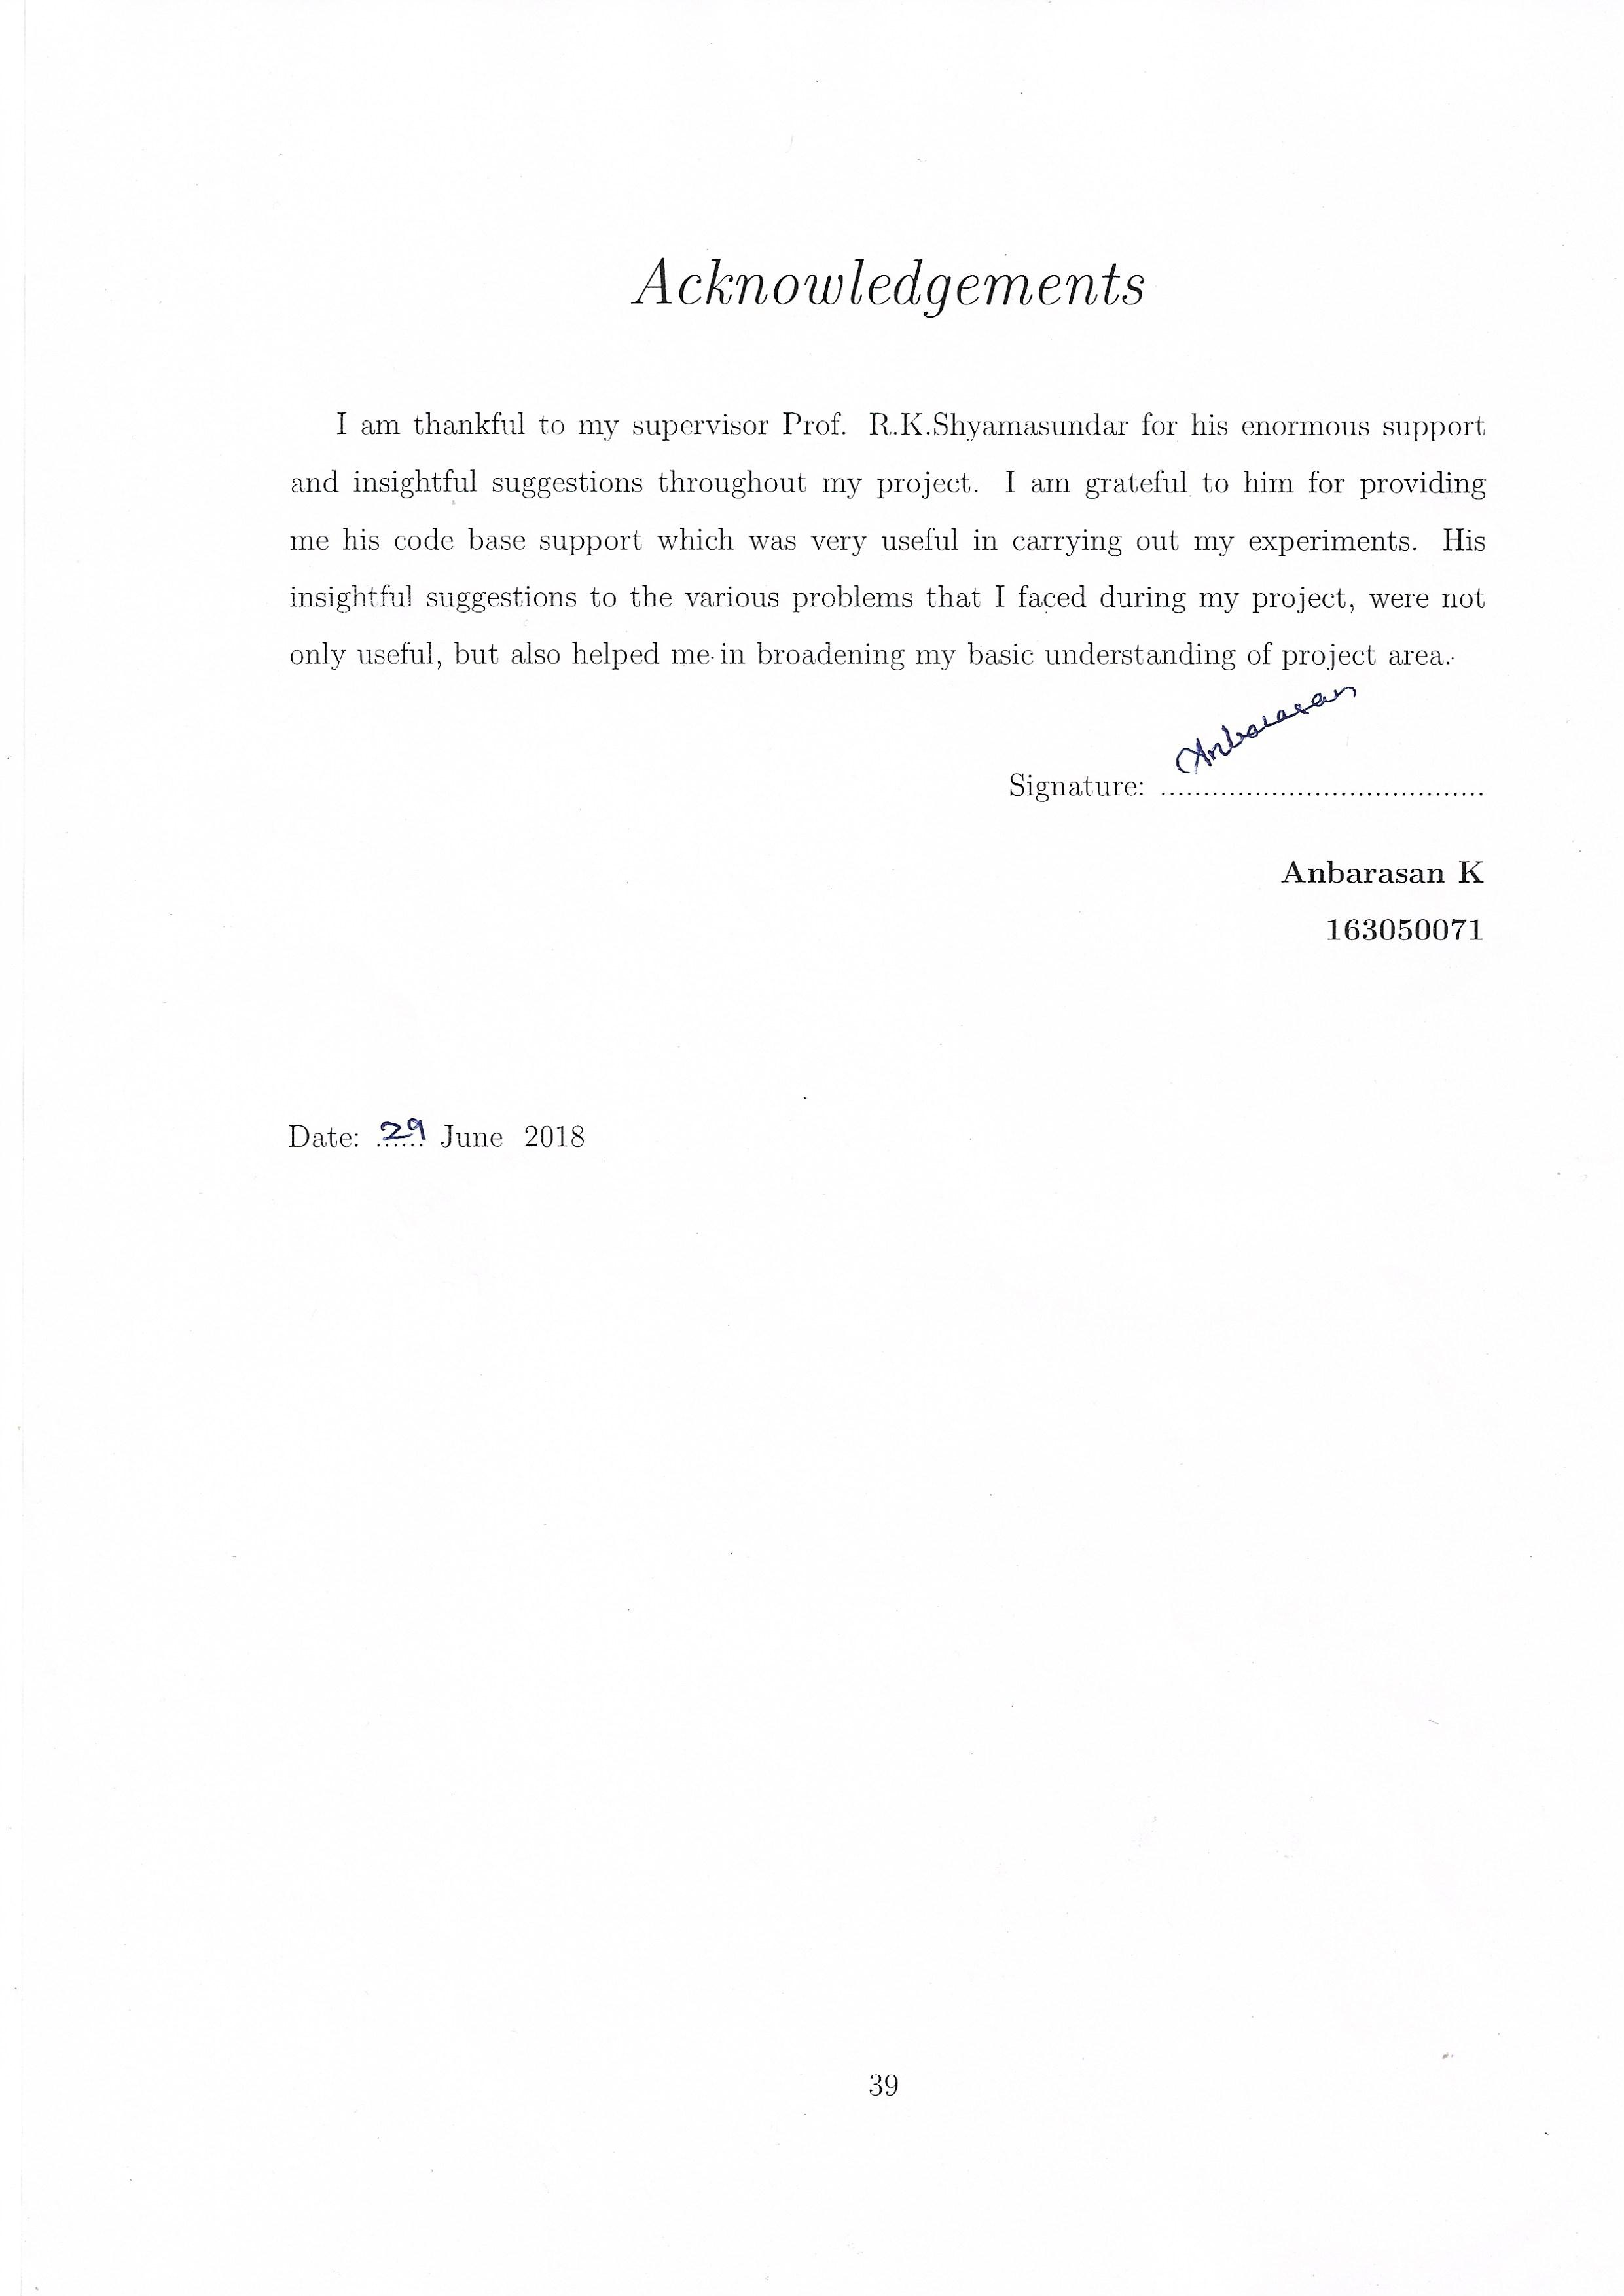
\includegraphics {Acknowledgement.jpg}}
\end{figure}
\restoregeometry
\clearpage

\end{document}
% End of the document